
\chapter{INTRODUCTION}

\section{Onion Routing}

As the prevalence of the Internet and other communication has grown, so too has the development and usage of privacy-enhancing systems. These are tools and protocols that provide privacy by obfuscating the link between a user's identification or location and their communications. Privacy is not achieved in traditional Internet connections because SSL/TLS encryption cannot hide IP and TCP headers, which must be exposed to allow routing between two parties; eavesdroppers can easily break user privacy by monitoring these headers. A closely related property is anonymity -- a part of privacy where user activities cannot be tracked and their communications are indistinguishable from others. Tools that provide these systems hold a user's identity in confidence, and privacy and anonymity are often provided together. Following a general distrust of unsecured Internet communications and in light of the 2013-current revelations by Edward Snowden of Internet mass-surveillance by the NSA, GCHQ, and other members of the Five Eyes, users have increasingly turned to these tools for their own protection. Privacy-enhancing and anonymity tools may also be used by the military, researchers working in sensitive topics, journalists, law enforcement running tip lines, activists and whistleblowers, or individuals in countries with Internet censorship. These users may turn to proxies or VPNs, but these tools often track their users for liability reasons and thus rarely provide anonymity. Furthermore, they can easily break confidence to destroy user privacy. More complex tools are needed for a stronger guarantee of privacy and anonymity.

Today, most anonymity tools descend from mixnets, a concept invented by David Chaum in 1981.\cite{chaum2003untraceable} In a mixnet, user messages are transmitted to one or more mixes, who each partially decrypt, scramble, delay, and retransmit the messages to other mixes or to the final destination. This enhances privacy by heavily obscuring the correlation between the origin, destination, and contents of the messages. Mixnets have inspired the development of many varied mixnet-like protocols and have generated significant literature within the field of network security.\cite{edman2009anonymity}\cite{syverson2011peel}

Mixnet descendants can generally be classified into two distinct categories: high-latency and low-latency systems. High-latency networks typically delay traffic packets and are notable for their greater resistance to global adversaries who monitor communication entering and exiting the network. However, high-latency networks, due to their slow speed, are typically not suitable for common Internet activities such as web browsing, instant messaging, or the prompt transmission of email. Low-latency networks, by contrast, do not delay packets and are thus more suited for these activities, but they are more vulnerable to timing attacks from global adversaries.\cite{dingledine2004tor} In this work, we detail and introduce new functionality within low-latency protocols.

Onion routing is a technique for enhancing privacy of TCP-based communication across a network and is the most popular low-latency descendant of mixnets in use today. It was first designed by the U.S. Naval Research Laboratory in 1997 for military usage \cite{syverson1997anonymous}\cite{reed1998anonymous} but has since seen widespread usage. In onion routing with public key infrastructure (PKI), a user selects a set network nodes, typically called \emph{onion routers} and together a \emph{circuit}, and encrypts the message with the public key of each router. Each encryption layer contains the next destination for the message -- the last layer contains the message's final destination. As the \emph{cell} containing the message travels through the network, each of these onion routers in turn decrypt their encryption layer like an onion, exposing their share of the routing information. The final recipient receives the message from the last router, but is never exposed to the message's source.\cite{syverson2011peel} The sender therefore has privacy because the recipient does not know the sender's location, and the sender has anonymity if no identifiable or distinguishing information is included in their message.

\begin{figure}[htbp]
	\centering
	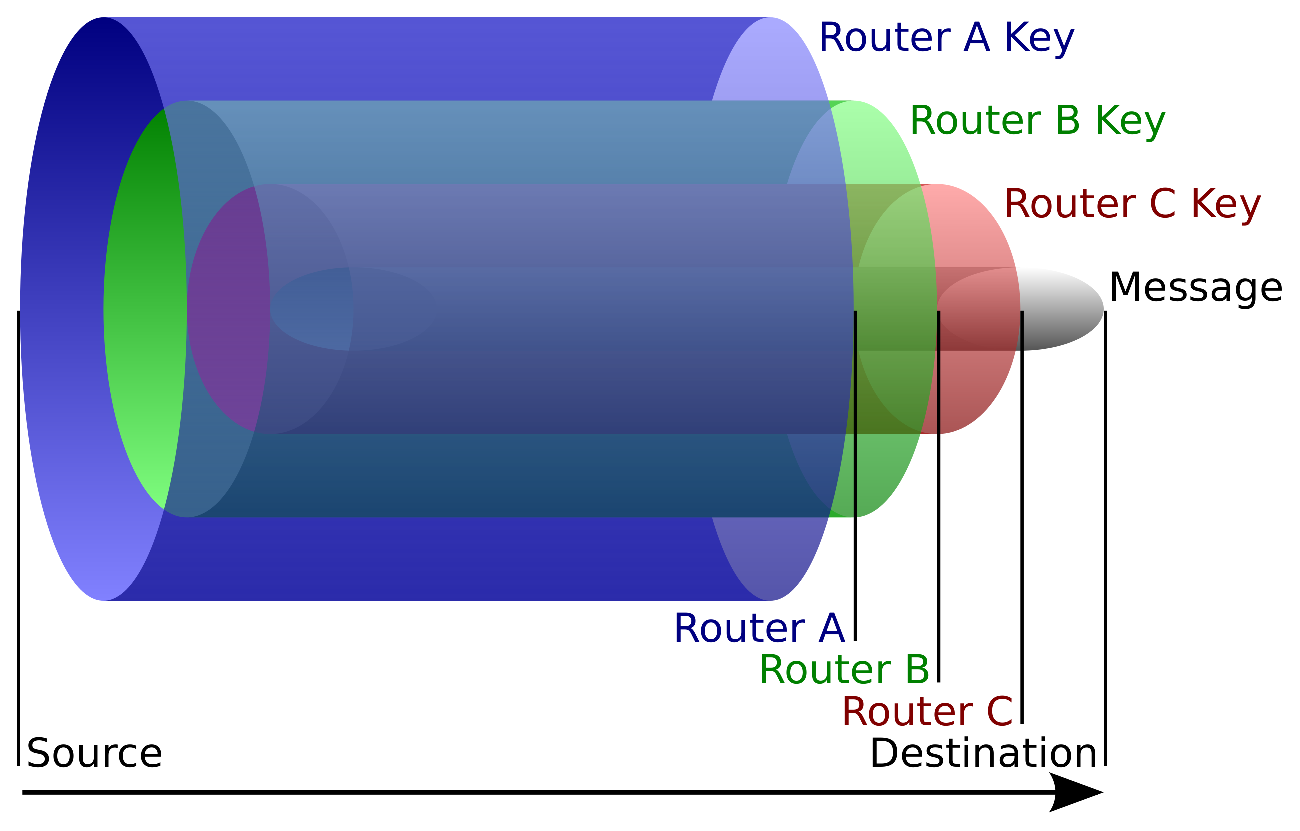
\includegraphics[width=0.5\textwidth]{images/onion-diagram.eps}
	\caption{An example cell and message encryption in an onion routing scheme. Each router ``peals'' off its respective layer of encryption; the final router exposes the final destination.}
\end{figure}

The first generation of onion routing used circuits fixed to a length of five, assumed a static network topology, and most notably, introduced the ability to mate two circuits at a common node or server. This last capability enabled broader anonymity where the circuit users were anonymous to each other and to the common server, a capability that was adopted and refined by later generation onion routers. Second generation introduced variable-length circuits, multiplexing of all user traffic over circuits, exit policies for the final router, and assumed a dynamic network by routing updates throughout the network. A client, Alice, in second-generation onion routers also distributed symmetric keys through the cell layers. If routers remember the destinations for each message they received, the recipient Bob can send his reply backwards through the circuit and each router re-encrypts the reply with their symmetric key. Alice unwraps all the layers, exposing the Bob's reply. The transition from public-key cryptography to symmetric-key encryption significantly reduced the CPU load on onion routers and enabled them to transfer more packets in the same amount of time. However, while influential, first and second generation onion routing networks have fallen out of use in favor of third-generation systems.\cite{syverson2011peel}

\section{Tor}

Tor is a third-generation onion routing system. It was invented in 2002 by Roger Dingledine, Nick Mathewson, and Paul Syverson of the Free Haven Project and the U.S. Naval Research Laboratory\cite{dingledine2004tor} and is the most popular onion router in use today. Tor inherited many of the concepts pioneered by earlier onion routers and implemented several key changes:\cite{syverson2011peel}\cite{dingledine2004tor}

\begin{itemize}
	\item \textbf{Perfect forward secrecy:} Rather than distributing keys via onion layers, Tor clients negotiate a TLS Diffie-Hellman-Merkle ephemeral key exchange with each of the routers in turn, extending the circuit one node at a time. These keys are then purged when the circuit is torn down; this achieves perfect forward secrecy, a property that ensures that the symmetric encryption keys will not be revealed if long-term public keys are later compromised.
	\item \textbf{Circuit isolation:} Second-generation onion routers mixed cells from different circuits in realtime, but later research could not justify this as an effective defence against an active adversary.\cite{syverson2011peel} Tor abandoned this in favor of isolating circuits from each other inside the network. Tor circuits are used for up to 10 minutes or whenever the user chooses to rotate to a fresh circuit.
	\item \textbf{Three-hop circuits:} Previous onion routers used long circuits to provide heavy traffic mixing. Tor removed mixing and fell back to using short circuits of minimal length. With three relays involved in each circuit, the first node (the \emph{guard}) is exposed to the user's IP address. The middle router passes onion cells between the guard and the final router (the \emph{exit}) and its encryption layer exposes it to neither the user's IP nor its traffic. The exit processes user traffic, but is unaware of the origin of the requests. While the choice of middle and exits can be routers can be safely random, the guard nodes must be chosen once and then consistently used to avoid a large cumulative chance of leaking the user's IP to an attacker. This is of particular importance for circuits from hidden services.\cite{bauer2007low}\cite{overlier2006locating}
	\item \textbf{Standardized to SOCKS proxy:} Tor simplified the multiplexing pipeline by transitioning from application-level proxies (HTTP, FTP, email, etc) to a TCP-level SOCKS proxy, which multiplexed user traffic and DNS requests through the onion circuit regardless of any higher protocol. The disadvantage to this approach is that Tor's client software has less capability to cache data and strip identifiable information out of a protocol. The countermeasure was the Tor Browser, a fork of Mozilla's open-source Firefox with a focus on security and privacy. To reduce the risks of users breaking their privacy through Javascript, it ships with the NoScript extension which blocks all web scripts not explicitly whitelisted. The browser also forces all web traffic, including DNS requests, through the Tor SOCKS proxy, provides a Windows-Firefox user agent regardless of the native platform, and includes many additional security and privacy enhancements not included in native Firefox. The browser also utilizes the EFF's HTTPS Everywhere extension to re-write HTTP web requests into HTTPS whenever possible; when this happens the Tor cell contains an additional inner encryption layer.
	\item \textbf{Directory servers:} Tor introduced a set of trusted directory servers to distribute network information and the public keys of onion routers. Onion routers mirror the digitally signed network information from the directories, distributing the load. This simplified approach is more flexible and scales faster than the previous flooding approach, but relies on the trust of central directory authorities. Tor ensures that each directory is independently maintained in multiple locations and jurisdictions, reducing the likelihood of an attacker compromising all of them.\cite{syverson2011peel} We describe the contents and format of the network information published by the directories in section \ref{sec:ConsensusDocs}.
	\item \textbf{Dynamic rendezvous with hidden services:} In previous onion routers, circuits mated at a fixed common node and did not use perfect forward secrecy. Tor uses a distributed hashtable to record the location of the introduction node for a given hidden service. Following the initial handshake, the hidden service and the client then meet at a different onion router chosen by the client. This approach significantly increased the reliability of hidden services and distributed the communication load across multiple rendezvous points.\cite{dingledine2004tor} We provide additional details on the hidden service protocol in section \ref{sec:HiddenServices} and our motivation for addition hidden service infrastructure in section \ref{sec:Motivation}.
\end{itemize}

As of March 2015, Tor has 2.3 million daily users that together generate 65 Gbit/s of traffic. Tor's network consists of nine authority nodes and 6,600 onion routers in 83 countries.\cite{TorMetrics} In a 2012 Top Secret presentation leaked by Edward Snowden, Tor was recognized by the U.S. National Security Agency as the "the king of high secure, low latency Internet anonymity".\cite{landau2014highlights} \cite{plak2014anonymous} In 2014, BusinessWeek claimed that Tor was ``perhaps the most effective means of defeating the online surveillance efforts of intelligence agencies around the world.''\cite{TorBusinessWeek}

\subsection{Design}

Tor's design focuses on being easily deployable, flexible, and well-understood. Tor also places emphasis on usability in order to attract more users; more user activity translates to an increased difficulty of isolating and breaking the privacy of any single individual. Tor however does not manipulate any application-level protocols nor does it make any attempt to defend against global attackers. Instead, its threat model assumes that the capabilities of adversaries are limited to observing fractions of Tor traffic, that they can actively delay, delete, or manipulate traffic, that they may attempt to digitally fingerprint packets, that they may run onion routers themselves, and that they may compromise a fraction of other existing routers. Together, most of the assumptions may be broadly classified as traffic analysis attacks. Tor's final focus is defending against these types of attacks.\cite{dingledine2004tor}

\subsection{Circuit Construction}

\emph{This section is incomplete. Here I will describe the Tor Authentication Protocol\cite{goldberg2006security}\cite{goldberg2013anonymity} which has since been extended to use ECDHE with ed25519 ECDSA: \cite{bernstein2006curve25519} and called NTor. I will walk through this protocol.}






%\begin{figure}[htdp]
%	\begin{minipage}[b]{0.45\linewidth}
%		\centering
%		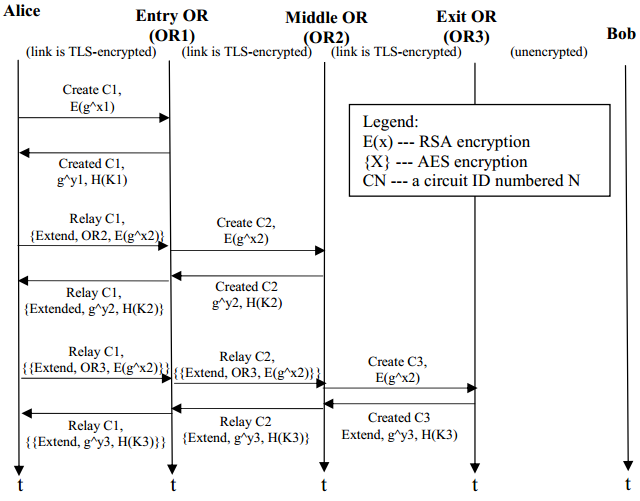
\includegraphics[width=\textwidth]{images/Tor/circuit-construction.png}
%		\caption{Anatomy of the construction of a Tor circuit.}
%		\label{fig:figure1}
%	\end{minipage}
%	\hspace{0.5cm}
%	\begin{minipage}[b]{0.45\linewidth}
%		\centering
%		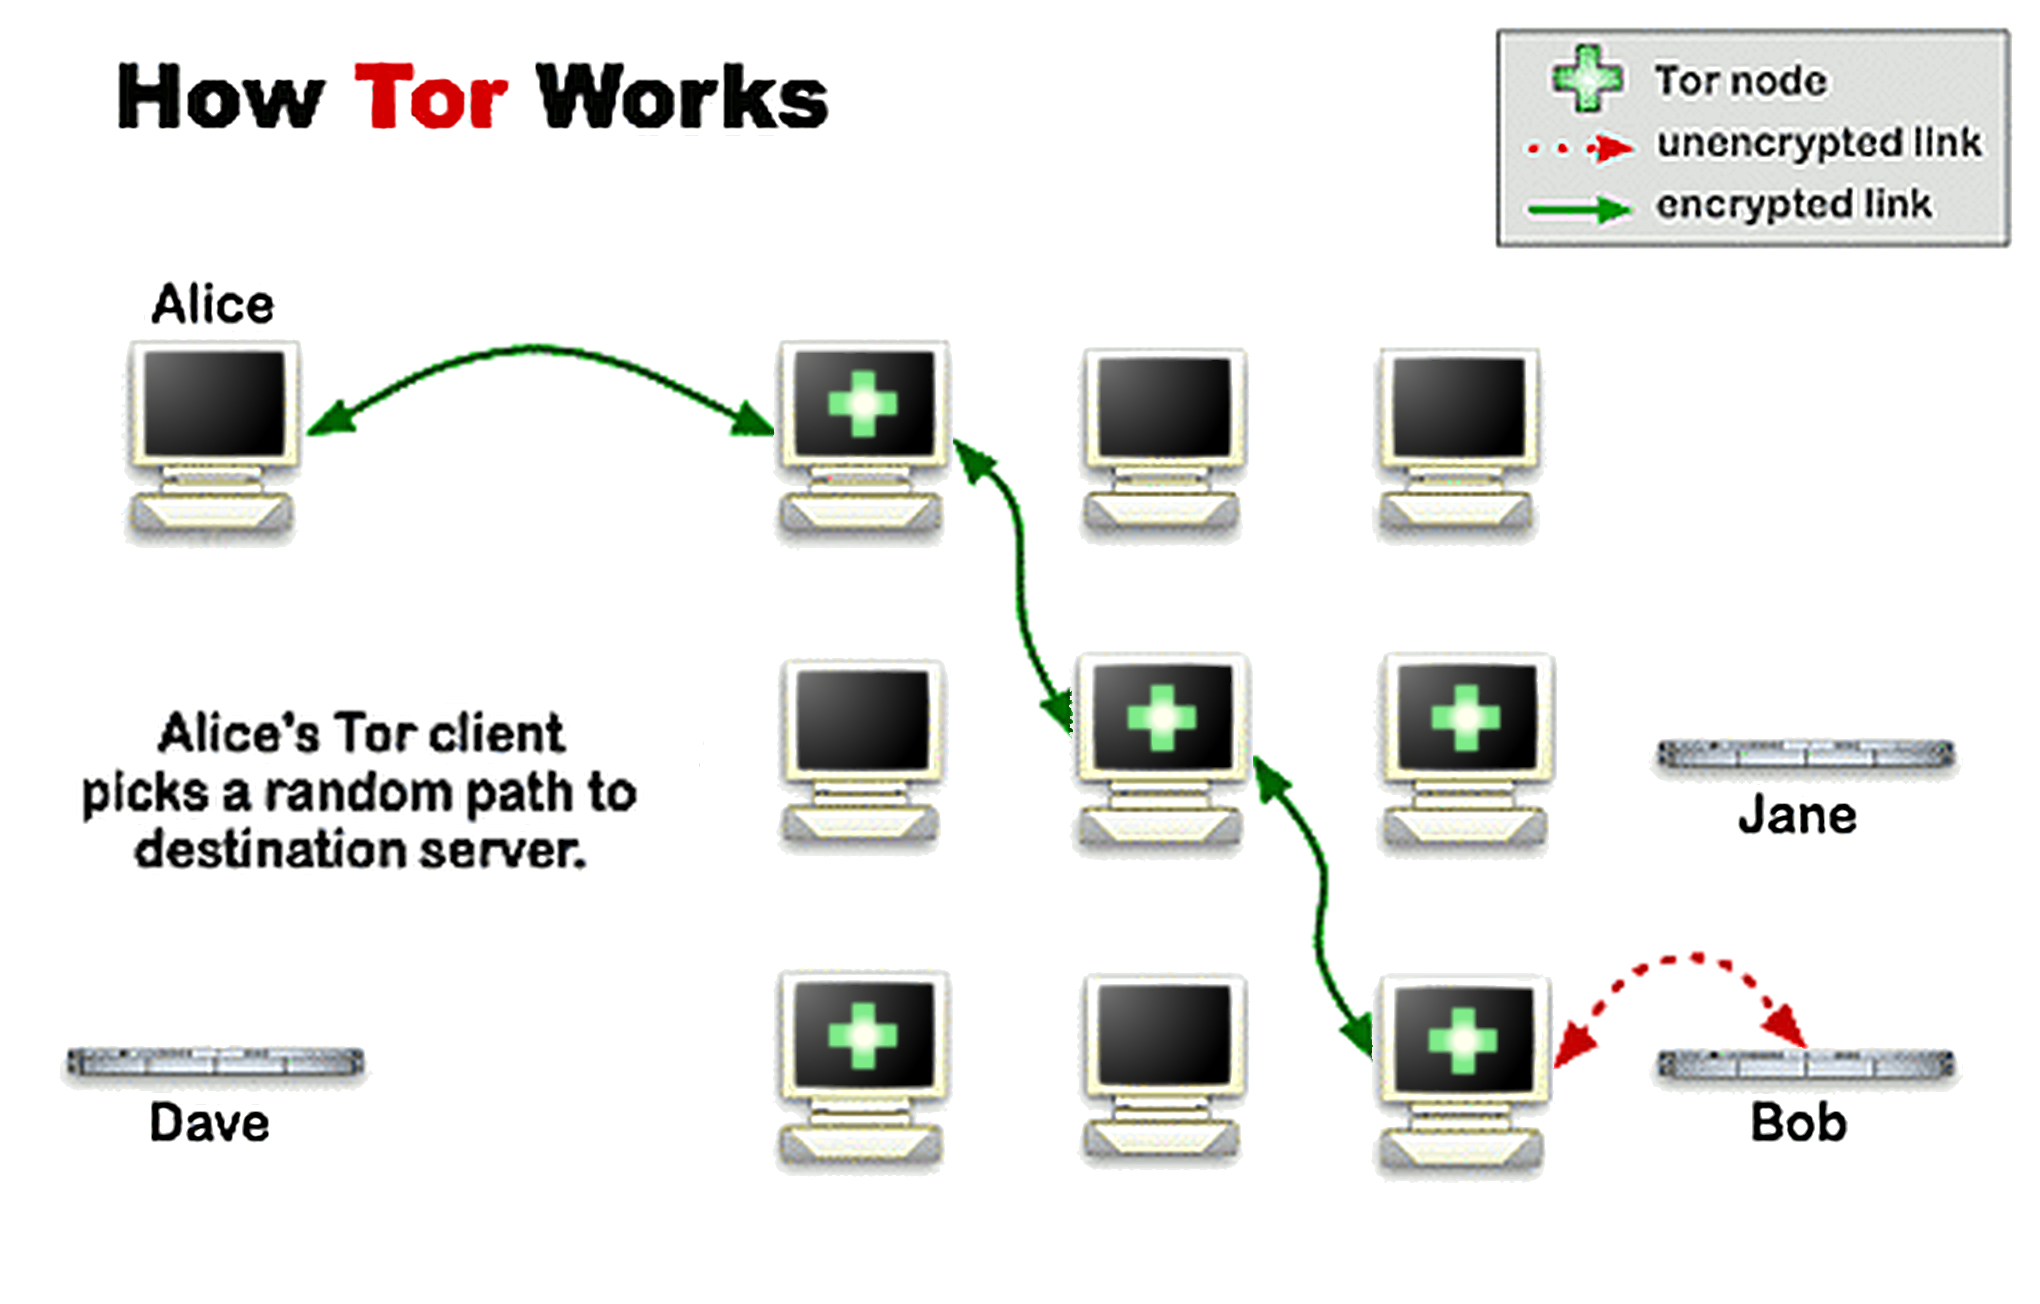
\includegraphics[width=\textwidth]{images/Tor/circuit-building-2-5.png}
%		\caption{A circuit through the Tor network.}
%		\label{fig:figure2}
%	\end{minipage}
%\end{figure}
%
%\textit{Todo: the following paragraph is not a complete description of Tor's crypto. I don't describe the NTor routing protocol.}
%
%The client first establishes a TLS connection with the first relay, $R_{1}$, using the relay's public key. The client then performs an ECDHE key exchange to negotiate $K_{1}$ which is then used to generate two symmetric session keys: a forward key $K_{1,F}$ and a backwards key $K_{1,B}$. $K_{1,F}$ is used to encrypt all communication from the client to $R_{1}$ and $K_{1,B}$ is used for all replies from $R_{1}$ to the client. These keys are used conjunction with the symmetric cipher suite negotiated during the TLS handshake, thus forming an encrypted tunnel with perfect forward secrecy. Once this one-hop circuit has been created, the client then sends $R_{1}$ the RELAY\_EXTEND command, the address of $R_{2}$, and the client's half of the Diffie-Hellman-Merkle protocol using $K_{1,F}$. $R_{1}$ performs a TLS handshake with $R_{2}$ and uses $R_{2}$'s public key to send this half of the handshake to $R_{2}$, who replies with his second half of the handshake and a hash of $K_{2}$. $R_{1}$ then forwards this to the client under $R_{1,B}$ with the RELAY\_EXTENDED command to notify the client. The client generates $K_{1,F}$ and $K_{1,B}$ from $K_{2}$, and repeats the process for $R_{3}$,\cite{ling2013protocol} as shown in Figure 3. The TCP/IP connections remain open, so the returned information travels back up the circuit to the end user.

At the application layer, this data is packed and padded into equally-sized Tor \textit{cells}, transmission units of 512 bytes. Tor further obfuscates user traffic by changing the circuit path every ten minutes,\cite{mccoy2008shining} as shown in Figure 4. A new circuit can also be requested manually by the user.

%\begin{figure}[htbp]
%	\centering
%	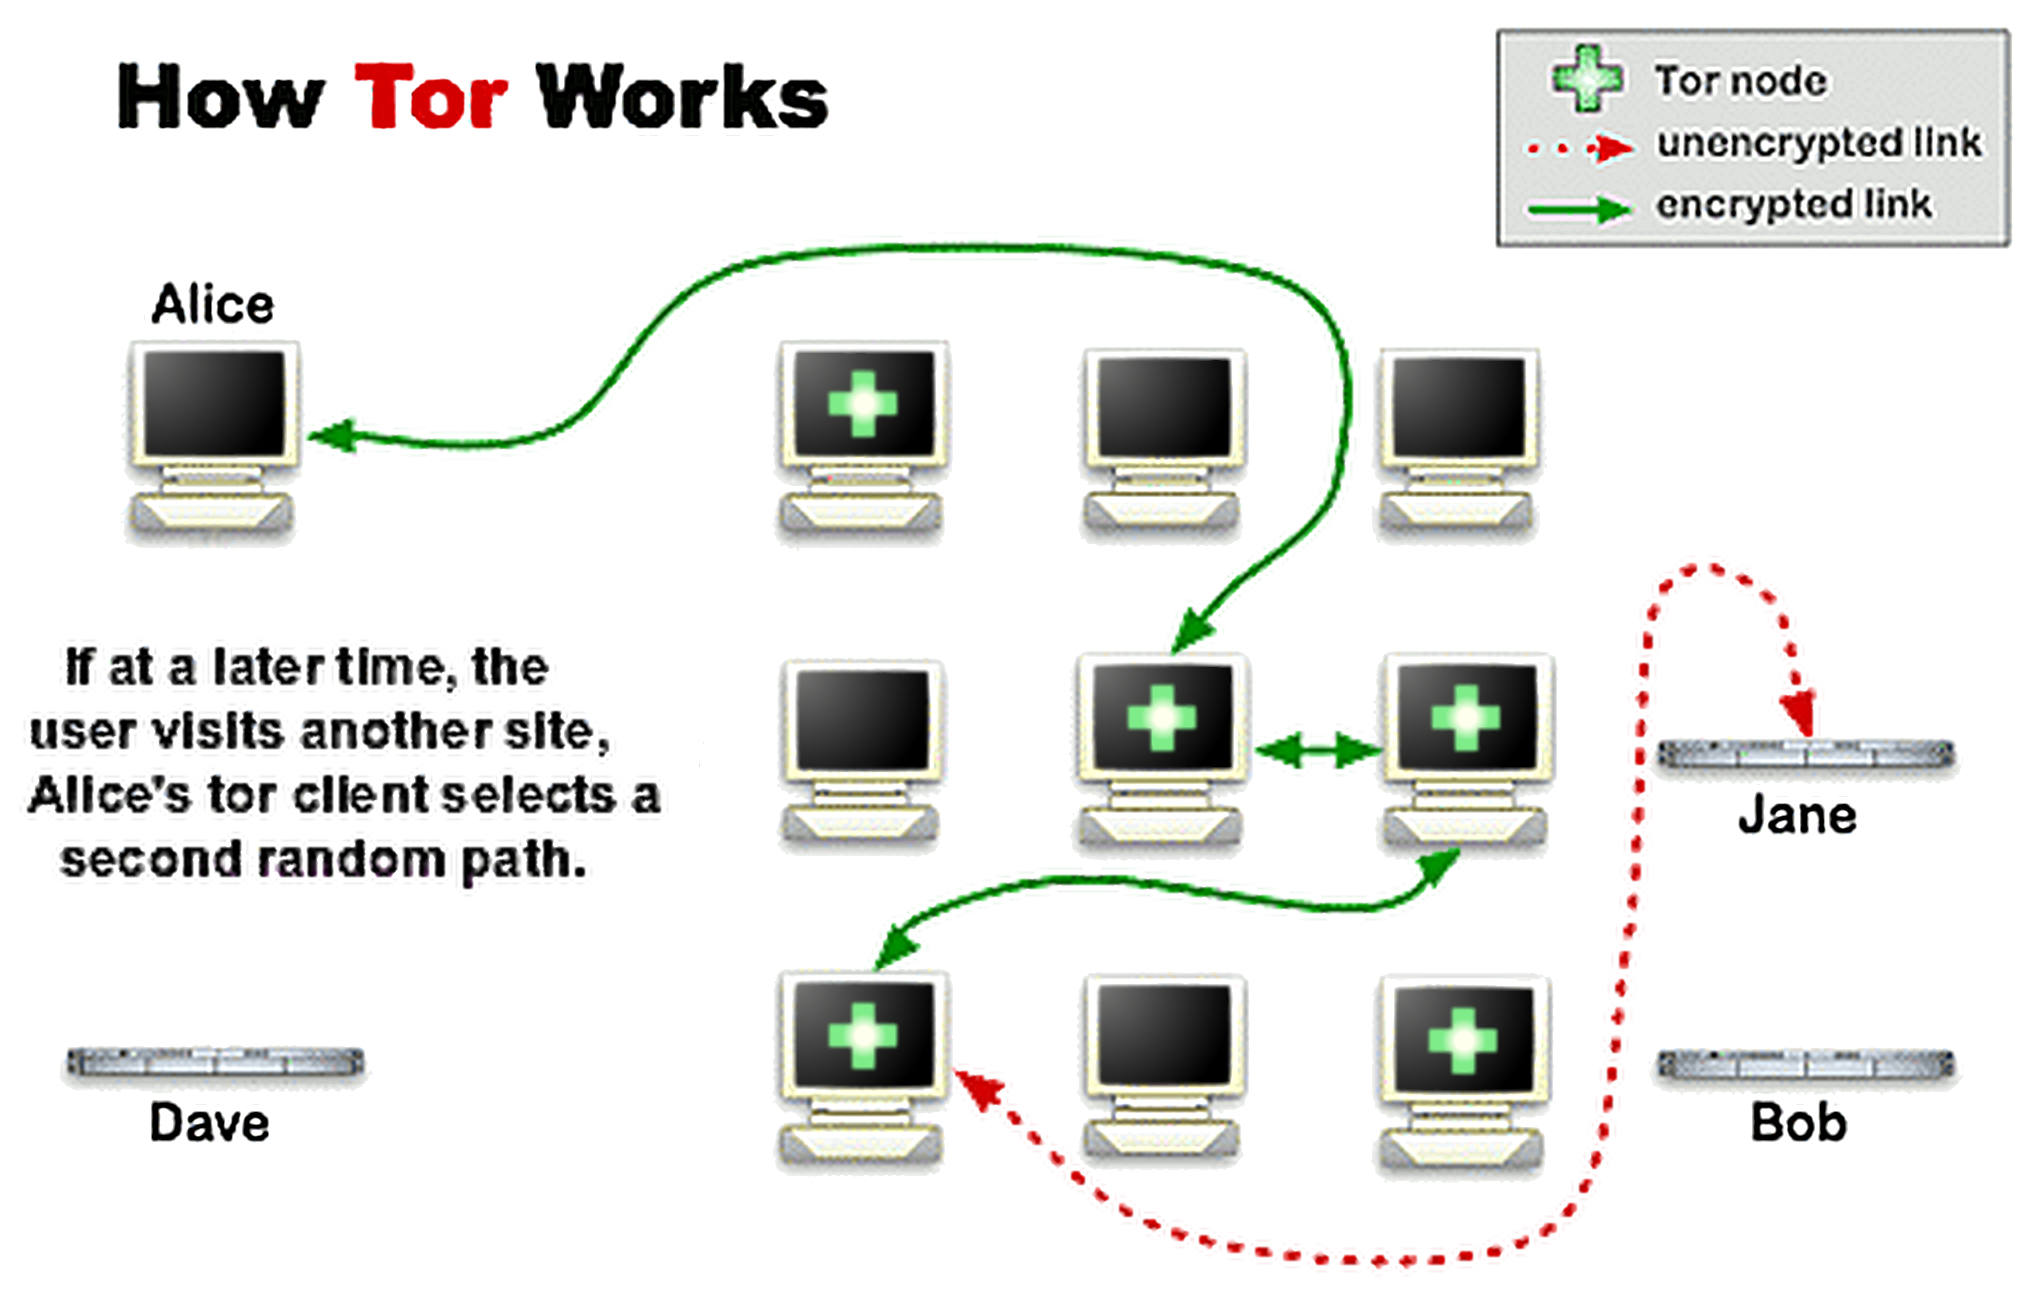
\includegraphics[width=0.6\textwidth]{images/Tor/circuit-change-1-4.png}
%	\caption{A Tor circuit is changed periodically, creating a new user identity.}
%\end{figure}
%
%% Although a different guard node is used here, in practice the choice of entry point is preserved for extended periods of time.
%
% If this happens, end-to-end encryption is complete and an outsider near the user would be faced with up to four layers of TLS encryption: $K_{1,F}(K_{2,F}(K_{3,F}(K_{server}(\textrm{client\ request}))))$ and likewise $K_{1,B}(K_{2,B}(K_{3,B}(K_{server}(\textrm{server\ reply}))))$ for the returning traffic, making traffic analysis very difficult.

\subsection{Consensus Documents}
\label{sec:ConsensusDocs}

The Tor network is maintained by nine authority nodes, who each vote on the status of nodes and together hourly publish a digitally signed consensus document containing IPs, ports, public keys, latest status, and capabilities of all nodes in the network. The document is then redistributed by other Tor nodes to clients, enabling access to the network. The document also allows clients to authenticate Tor nodes when constructing circuits, as well as allowing Tor nodes to authenticate one another. Since all parties have prior knowledge of the public keys of the authority nodes, the consensus document cannot be forged or modified without disrupting the digital signature.\cite{xin2009design}

\emph{Here I plan to detail the consensus documents that I will be using, since I use them in my Solution section.}

\subsection{Hidden Services}
\label{sec:HiddenServices}

Although Tor's primary and most popular use is for secure access to the traditional Internet, since 2004 Tor also supports anonymous services, such as websites, marketplaces, or chatrooms. These are a part of the Dark Web and cannot be normally accessed outside the context of Tor. In contrast to Tor-anonymized web requests where the client is anonymous but the server is known, Tor hidden services provide bidirectional anonymity where both parties remain anonymous and never directly communicate with one another. This allows for a greater range of communication capabilities.\cite{nicolussi2011human}

Tor hidden services are known only by their public RSA key. Tor does not contain a DNS system for its websites; instead the domain names of hidden services are an 80-bit truncated SHA-1 hash of its public key, postpended by the .onion top-level domain (TLD). Once the hidden service is contacted and its public key obtained, this key can be checked against the requested domain to verify the authenticity of the service server. This process is analogous to SSL certificates in the clearnet, however Tor's authenticity check leaks no identifiable information about the anonymous server. If a client obtains the hash domain name of the hidden service through a backchannel and enters it into the Tor Browser, the hidden service lookup begins.

Preceding any client communication, the hidden server, Bob, first builds Tor circuits to several random relays and enables them to act as \textit{introduction points} by giving them its public key, $ B_{K} $. The server then uploads its public key and the fingerprint identity of these nodes to a distributed hashtable inside the Tor network, signing the result. When a client, Alice, requests contact with Bob, Alice's Tor software queries this hashtable, obtains $ B_{K} $ and Bob's introduction points, and builds a Tor circuit to one of them, $ ip_{1} $. Simultaneously, the client also builds a circuit to another relay, $ rp $, which she enables as a rendezvous point by telling it a one-time secret, $ sec $. During this procedure, hidden services must continue to use their same entry node in order to avoid leaking its IP address to possibly malicious onion routers.\cite{bauer2007low}\cite{overlier2006locating}

\begin{figure}[htdp]
	\begin{minipage}[b]{0.45\linewidth}
		\centering
		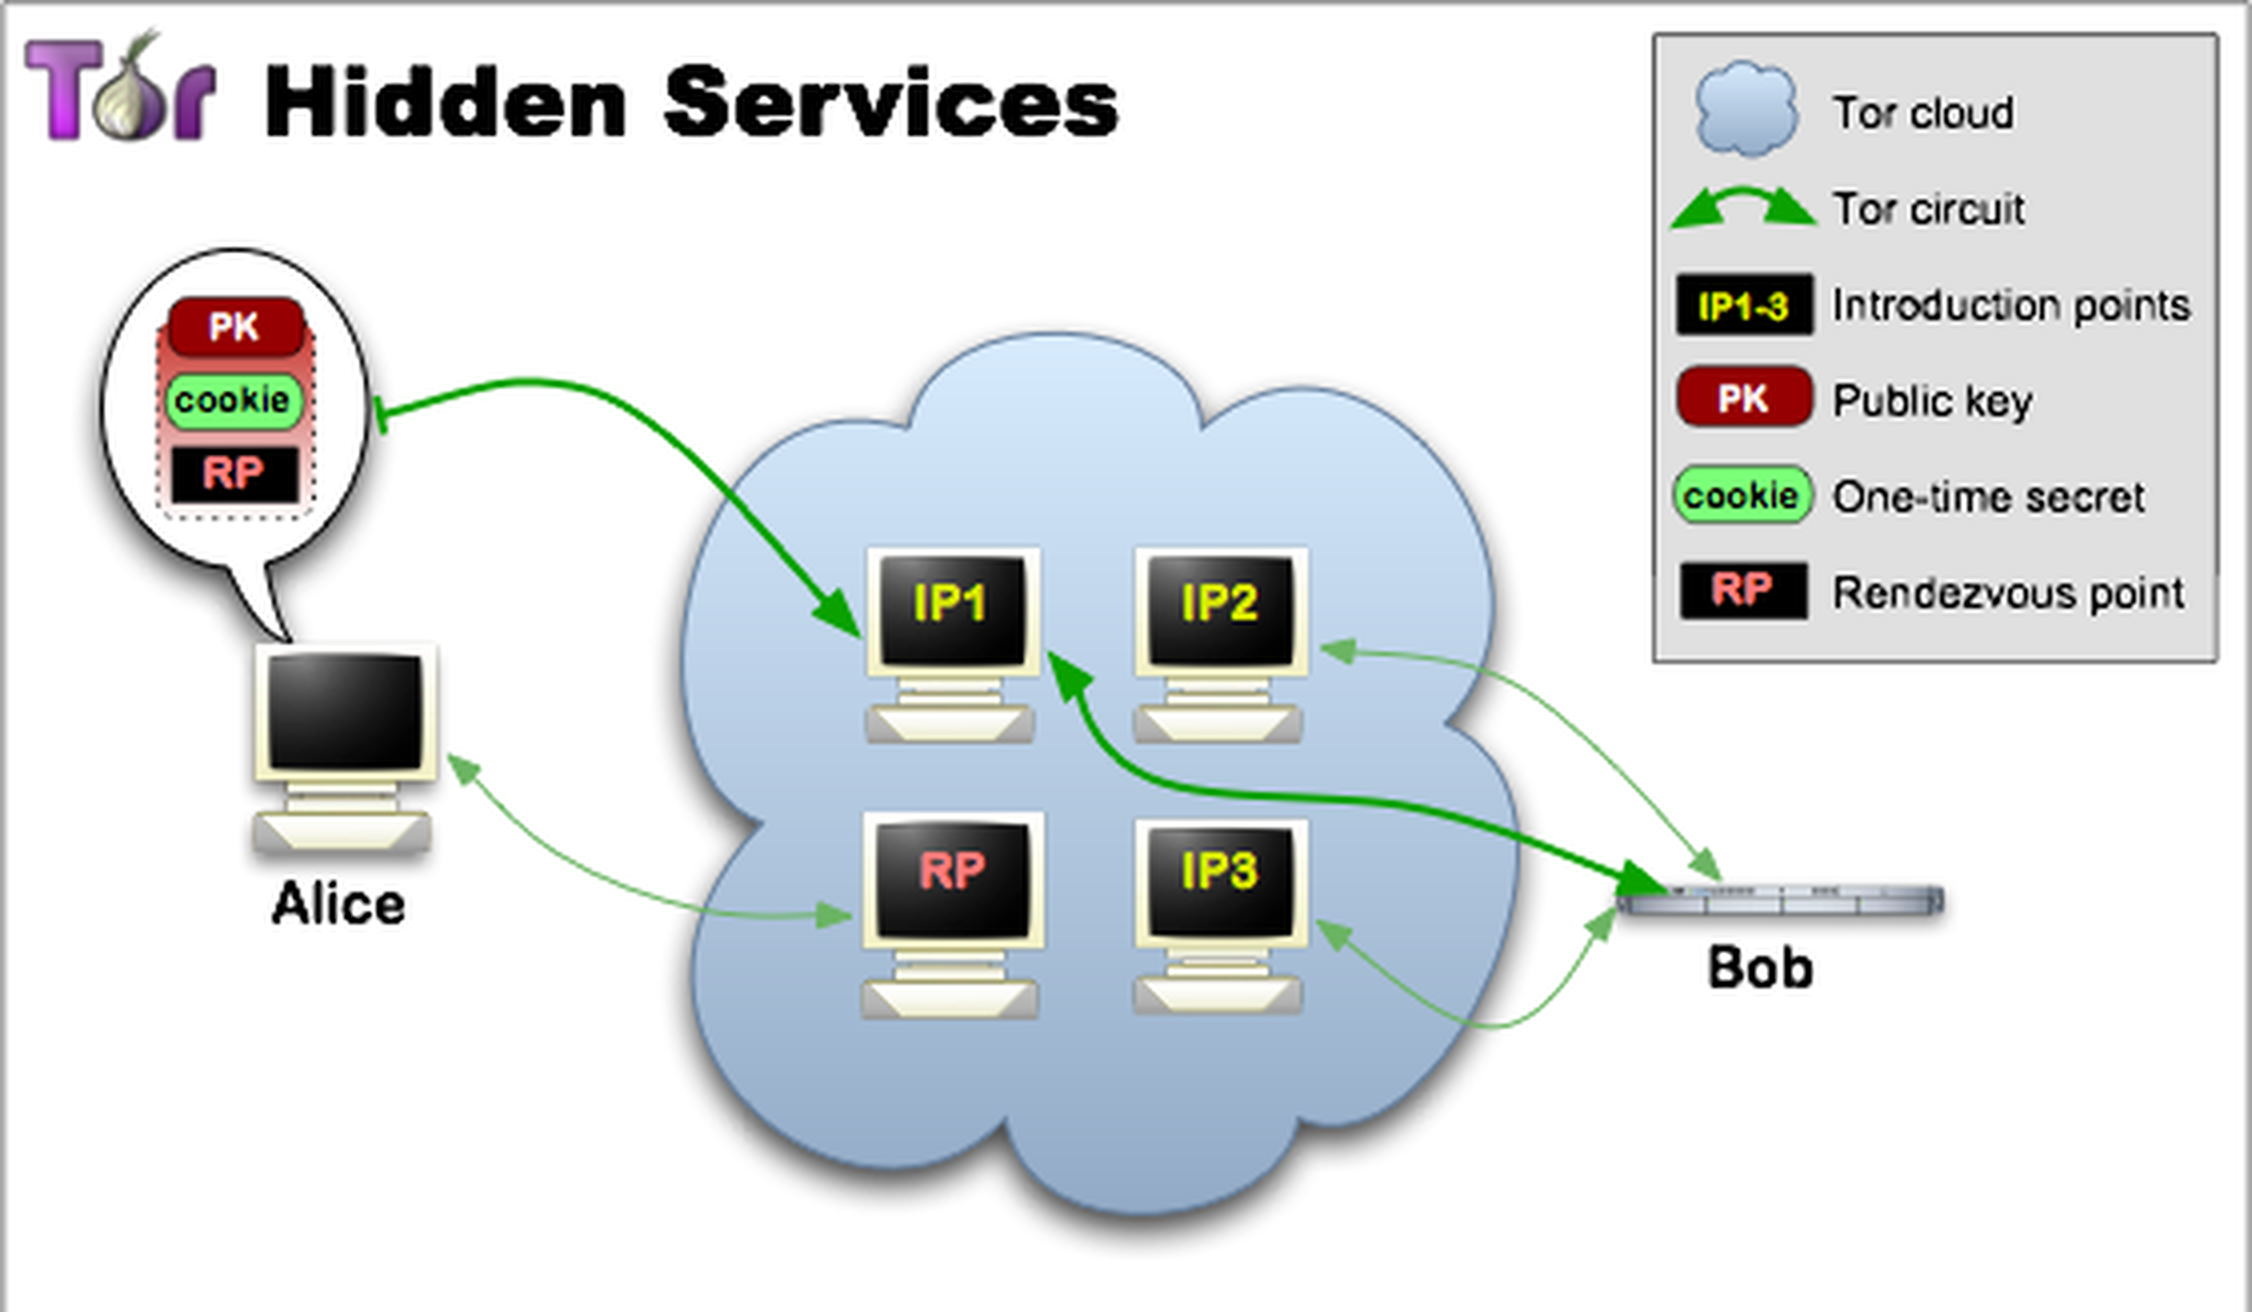
\includegraphics[width=\textwidth]{images/Tor/tor-hidden-service-4-higher.png}
		\caption{Alice uses the encrypted cookie to tell Bob to switch to $ rp $.}
	\end{minipage}
	\hspace{0.5cm}
	\begin{minipage}[b]{0.45\linewidth}
		\centering
		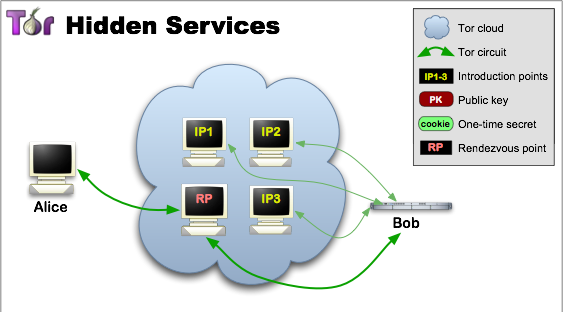
\includegraphics[width=\textwidth]{images/Tor/tor-hidden-service-6.png}
		\caption{Bidirectional communication between Alice and the hidden service.}
	\end{minipage}
\end{figure}

She then sends to $ ip_{1} $ a cookie encrypted with $ B_{K} $, containing $ rp $ and $ sec $. Bob decrypts this message, builds a circuit to $ rp $, and tells it $ sec $, enabling Alice and Bob to communicate. Their communication travels through six Tor nodes: three established by Alice and three by Bob, so both parties remain anonymous. From there traditional HTTP, FTP, SSH, or other protocols can be multiplexed over this new channel.

\section{Motivation}
\label{sec:Motivation}

The usability of hidden services is severely challenged by their non-intuitive 16-character base58-encoded domain names. To choose several prominent examples, 3g2upl4pq6kufc4m.onion is the address for the DuckDuckGo hidden service, 33y6fjyhs3phzfjj.onion is the Guardian's SecureDrop service for anonymous document submission, and blockchainbdgpzk.onion is the anonymized edition of blockchain.info. It is rarely clear what service a hidden server is providing by its domain name alone without relying on third-party directories for the correlation, directories which must be updated and reliably maintained constantly. These must be then distributed through backchannels such as /r/onions, the-hidden-wiki.com, or through a hidden service that is known in advance. It is a frequent topic of conversation inside Tor communities. It is clear that this problem limits the usability and popularity of Tor hidden services. Although there have been some workarounds that are partially successful, the issue remains unresolved. It is for these reasons that I propose OnionNS as a full solution.

\section{Contributions}


